\documentclass[12pt]{article}
\usepackage{graphicx}
\usepackage {color}
\usepackage{pdfpages}
\usepackage{float}
\usepackage{changebar}
\usepackage{enumitem,amssymb}
\renewcommand{\familydefault}{\sfdefault}
\usepackage[margin=1.2in]{geometry}
\usepackage{graphicx}
\usepackage{wrapfig}
\usepackage[super]{cite}
\usepackage{subcaption}
\usepackage[table]{xcolor}
\usepackage{amsmath}
\usepackage[sort, numbers]{natbib}
\usepackage{multirow}
\usepackage{tabularx}
\usepackage{siunitx}
\usepackage{matlab-prettifier}
\usepackage{wrapfig,lipsum,booktabs}
%%%%%%%%%%%%Defining the margins %%%%%%%%%%%%%%%%%%%%%
\textheight 9.in
\textwidth 6.5in
\topmargin -.5in
\oddsidemargin 0in
\setlength{\parskip}{\smallskipamount}

%%%%%%%%%%%%%%Specific Commands %%%%%%%%%%%%%%%%%%
\newcommand{\eg}{{\em e.g.,}}
\newcommand{\ie}{{\em i.e.,}}
\newcommand{\etc}{{\em etc.,}}
\newcommand{\etal}{{\em et al.}}
\newcommand{\degrees}{{$^{\circ}$}}
\newcommand{\fig}[1]{\textbf{Figure #1}}

%%%%%%%%%%%%%%%%%%%%%%%%%%%% Setting to control figure placement
% These determine the rules used to place floating objects like figures 
% They are only guides, but read the manual to see the effect of each.
\renewcommand{\topfraction}{.9}
\renewcommand{\bottomfraction}{.9}
\renewcommand{\textfraction}{.1}
\renewcommand{\familydefault}{\sfdefault} %setting the san serif font

%%%%%%%%%%%%%%%%%%%%%%%% Line spacing
% Use the following command for ``double'' spacing
%\setlength{\baselineskip}{1.2\baselineskip}
% and this one for an acceptable NIH spacing of 6lpi based on 11pt
%\setlength{\baselineskip}{.9\baselineskip}
% The baselineskip does not appear to work when we include a maketitle
% command in the main file.  Something there must set the line spacing
% If we use this next command, then things seem to work.
\renewcommand{\baselinestretch}{.9}

\setcounter{secnumdepth}{0} %make no numbers but have a table of contents


\begin{document}

\title{HW 4: Medical Imaging Systems}
\author{Jake Bergquist, u6010393 }
\maketitle

\section{Q1}
\noindent\textbf{a: } Attached is the sketch of the emission spectrum for the element in question. Using these K, L, and M bining energies we calculate a $K_\alpha = 22.0 keV$, a $K_\beta = 24.4 keV$, and $L_\alpha = 2.4 meV$. The $L_\alpha$ peak is filtered out by the $10 keV$ filter assumed in the problem statement. Thus with a $30 keV$ source we get the usual emission spectrum shape with a peak at the $K_\alpha$ and $K_\beta$ energies. Also shown in dotted lines is the shape of the emission curve without the filtering.

\noindent\textbf{b: } Attached is the sketch of the emission spectrum with additional filtering by the element. First of all we know that there will be a decreased emission due to the general blanket absorption of the element. Additionally the element will have sharp spikes in absorption at its K, L, and M binding energies. The absorption profile for this element is shown in the attached figure. The L and M shelves are below the 1$10keV$ filter and thus will have no effect but the K binding energy of $25 keV$ will cause a K shelf to be seen int he emission spectrum when filtered by this element, sharply filtering our energies at or above this energy.

\section{Q2}
\noindent\textbf{a: } 
For a given number of photons that enter a material, $N_{in}$, we know that the number of photons leaving that material, $N_{out}$, is given by Eq~\ref{eq3} below where $\mu$ is the mass attenuation coefficient of the material and $t$ is the thickness of the tissue.
 \begin{equation}
 N_{out} = N_{in}e^{-\mu t}
 \label{eq3}
 \end{equation}
\noindent Additionally we know that the intensity of the x-ray beam is given by $I = NE$ where $N$ is the number of photons and $E$ is the energy. Additionally we know that the number of photons, $N$, can be expressed as $N = A_{roi}\lambda$ where $A_{roi}$ is the area of the region of interest and $\lambda$ is the fluence of the source. Using these relationships and Eq~\ref{eq3} we can get an expression for each of our beam intensities. For $beam_2$ this is easy because here is only one mass attenuation coefficient and one tissue thickness thus:\\ $I_{beam2} = EA_{roi}\lambda e^{-\mu_{tissue}t_{tissue}}$\\ For $beam_1$ we have two tisssues (tissue and vessle) and the two thicknesses. Thus our expression becomes \\$I_{beam1} =EA_{roi}\lambda e^{-\mu_{vessel}t_{vessel}}e^{-\mu_{tissue}(t_{tissue}-t_{vessel})}$\\

\noindent\textbf{b: }
The equation for $beam_2$ is unchanged with the contrast. The equation for $beam_1$ becomes:\\
$I_{beam1} =EA_{roi}\lambda e^{-\mu_{contrast}t_{vessel}}e^{-\mu_{tissue}(t_{tissue}-t_{vessel})}$\\

\noindent\textbf{c: }
Let us first consider the case with $beam_1$. We have $I_0^1$ which is the intensity of $beam_1$ without contrast and $I_c^1$ which is the intensity with contrast. If we divide one by the other, say $I_C^1$ by $I_0^1$ we see that most of the tems cancel out and we are left with two exponentials relating the attenuation coefficients of the vessle and the contrast as below:\\
$\frac{I_c^1}{I_0^1} = \frac{EA_{roi}\lambda e^{-\mu_{contrast}t_{vessel}}e^{-\mu_{tissue}(t_{tissue}-t_{vessel})}}{EA_{roi}\lambda e^{-\mu_{vessel}t_{vessel}}e^{-\mu_{tissue}(t_{tissue}-t_{vessel})}} = \frac{e^{-\mu_{contrast}t_{vessel}}}{e^{-\mu_{vessel}t_{vessel}}}$

\section{Q3}

\section{Q4}
First we want to figure out what the exposure is at the lungs that would lead to a dose of 10 mrems = 0.01R. To do so we can use the relationship shown in Eq~\ref{eq1} that relates Dose ($D$) to Exposure ($X$).
\begin{equation}
D = \frac{0.873(\frac{\mu}{\rho})_{tissue}}{(\frac{\mu}{\rho})_{air}}X
\label{eq1}
\end{equation}
\noindent We can then check the National Institute of Standards and Technology (NIST) which keeps a database for the mass attenuation coefficients of various materials at various energies. At $50keV = 5\cdot10^{-2}MeV$ we find that dry air near sea level (which we assume to be our case) has a mass attenuation coefficient of $(\frac{\mu}{\rho})_{air} = 0.2080\frac{cm^2}{g}$. For lung tissue we find that at $50keV$ we get a mass attenuation of $(\frac{\mu}{\rho})_{lung} = 0.2270\frac{cm^2}{g}$. Substituting these into [\ref{eq1}] and solving for X we get an exposure of $X = \frac{D(\frac{\mu}{\rho})_{air}}{0.873(\frac{\mu}{\rho})_{lung} } = \frac{0.01 R \cdot 0.2080\frac{cm^2}{g}}{0.873\cdot 0.2270\frac{cm^2}{g}} = 0.0105 R$. 

\noindent Now we know what the exposure needs to be at the location of the lungs. Using this and our knowledge of what the exposure is 1cm from the source (10R) we can find out how far from the source we need to be in order to get  our desired exposure. To do so we use the inverse square law to determine what the distance to get this exposure is. Eq~\ref{eq2} shows us this relationship. By plugging in $1cm$ for $D_1$, $10R$ for $X_1$, and $0.0105R$ for $X_2$ then solving for $D_2$ we get our desired distance.
\begin{equation}
\frac{D_1^2}{D_2^2} = \frac{X_2}{X_1}
\label{eq2}
\end{equation}


\noindent $D_2 = \sqrt{\frac{D_1^2X_1}{X_2}} = \sqrt{\frac{1cm^2\cdot 10R}{0.0105R}} = 30.9 cm$ We can rework this entire formulation, instead solving for the Dose delivered at 1 cm then using the inverse square to calculate at what distance this dose falls off to the desired 10 mrem, and doing so yields the same answer of 30.9 cm. Thus to be safe I would recommend placing the lungs of the patient at least 31 cm from the source. 
\section{Q5}

\end{document}



\begin{figure}[H]
	\centering
	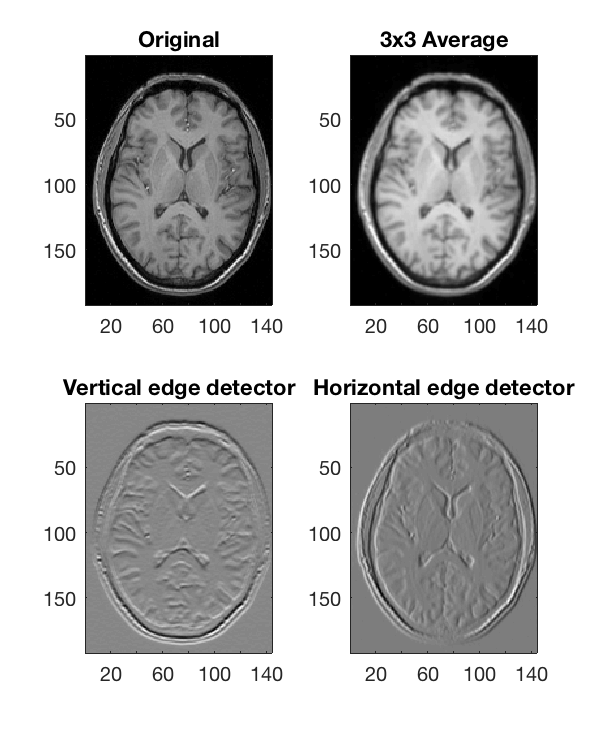
\includegraphics[width=\textwidth]{Figures/convs.png}
	\caption{}
	\label{Fig:conv}
\end{figure}

\begin{lstlisting}[style=Matlab-editor]

\end{lstlisting}




